\documentclass[tikz,border=10pt]{standalone}
\usepackage[T1]{fontenc}
\usepackage{times}
\usepackage{amssymb}
\usetikzlibrary{positioning,arrows.meta,fit,backgrounds,calc}

\begin{document}
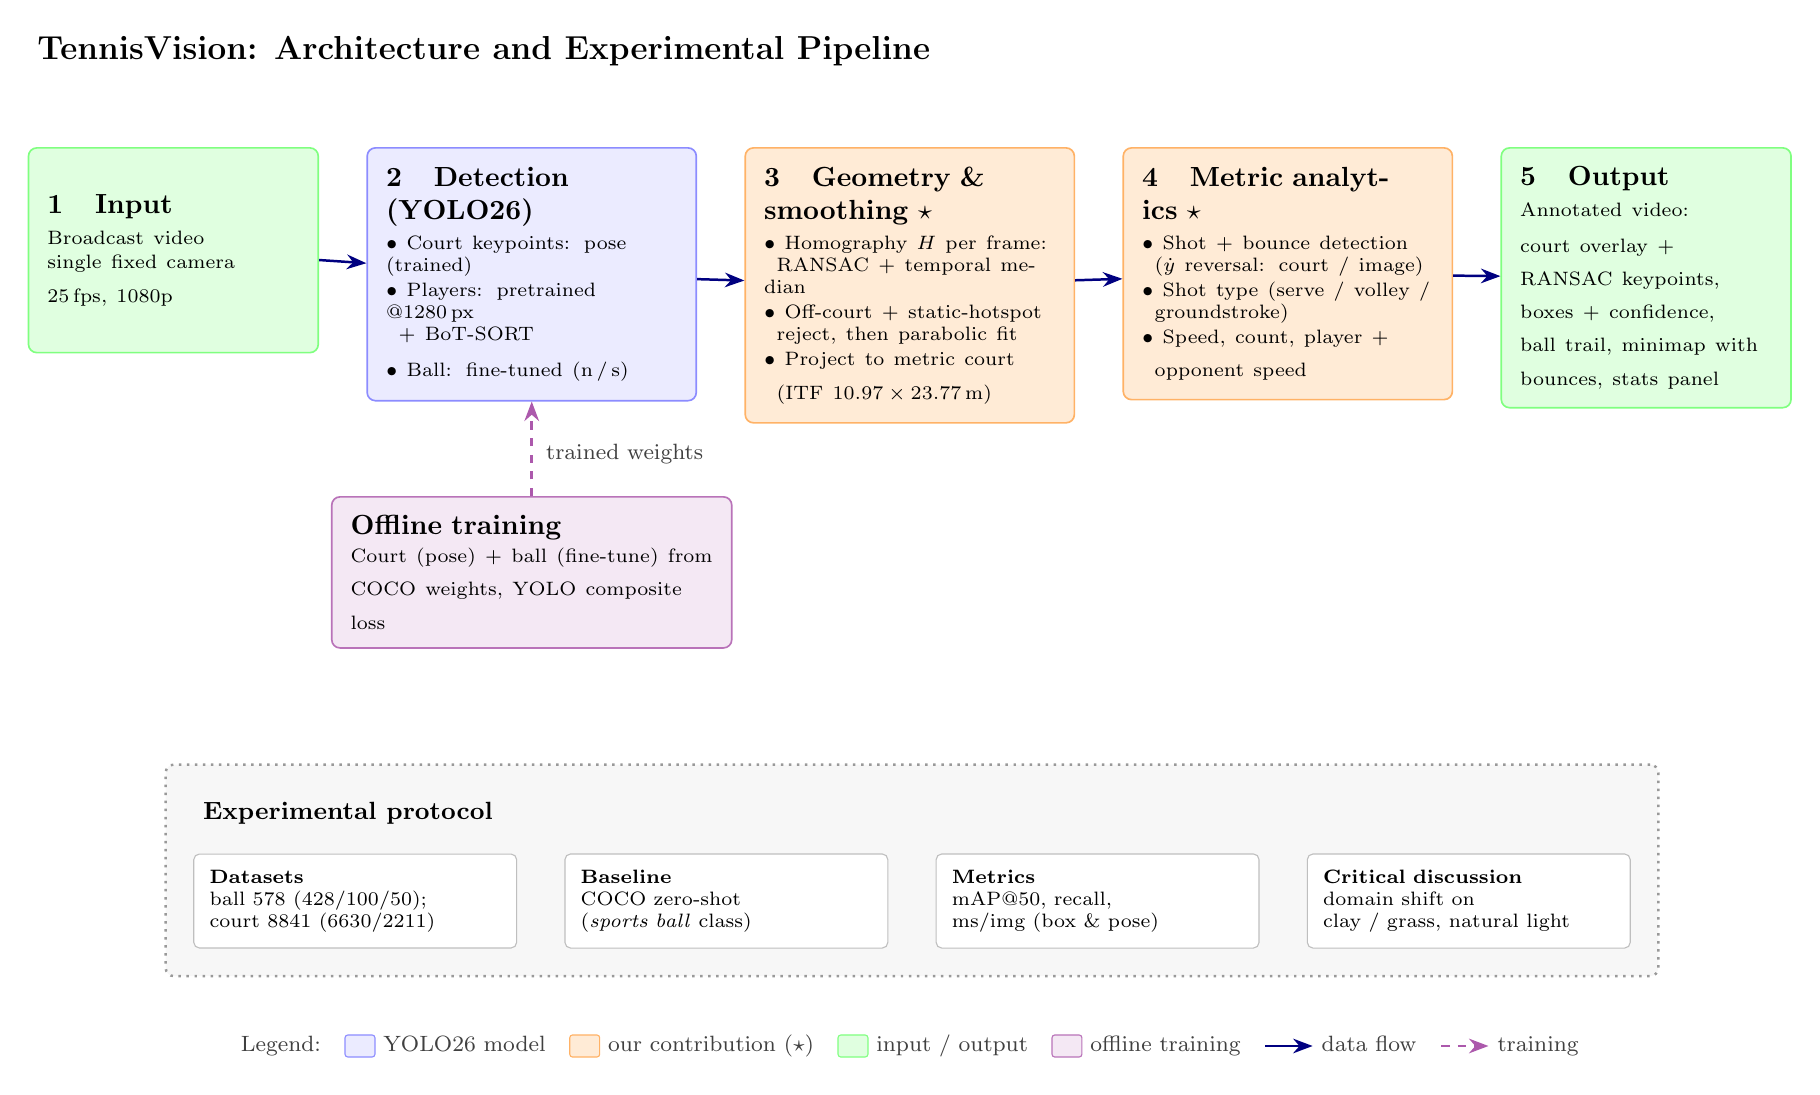
\begin{tikzpicture}[
	font=\rmfamily,
	>=Stealth,
	stage/.style={draw=blue!45, line width=0.6pt, rounded corners=3pt,
		align=left, text width=37mm, minimum height=26mm, inner sep=2.4mm,
		fill=blue!8},
	contrib/.style={stage, fill=orange!16, draw=orange!60},
	io/.style={stage, fill=green!12, draw=green!50, text width=32mm},
	aux/.style={draw=violet!55, line width=0.6pt, rounded corners=3pt,
		align=left, text width=46mm, inner sep=2.4mm, fill=violet!9},
	pit/.style={draw=black!25, rounded corners=2pt, align=left,
		text width=37mm, inner sep=2mm, fill=white, font=\scriptsize},
	hd/.style={font=\rmfamily\bfseries\small},
	flow/.style={->, line width=0.9pt, blue!50!black},
	train/.style={->, line width=0.9pt, dashed, violet!65},
	lgtxt/.style={font=\rmfamily\footnotesize, text=black!75},
]

% ---- title ----
\node[hd, font=\rmfamily\bfseries\large] (title) {TennisVision: Architecture and Experimental Pipeline};

% ---- main pipeline row (tops aligned) ----
\node[io, below=9mm of title.south west, anchor=north west] (in)
	{\textbf{1\quad Input}\\[3pt]
	 {\scriptsize Broadcast video\\[1pt] single fixed camera\\ 25\,fps, 1080p}};

\node[stage, anchor=north west] (det) at ([xshift=6mm]in.north east)
	{\textbf{2\quad Detection (YOLO26)}\\[3pt]
	 {\scriptsize $\bullet$~Court keypoints: pose (trained)\\[1pt]
	  $\bullet$~Players: pretrained @1280\,px\\ \hspace*{1.6mm}+ BoT-SORT\\[1pt]
	  $\bullet$~Ball: fine-tuned (n\,/\,s)}};

\node[contrib, anchor=north west] (geo) at ([xshift=6mm]det.north east)
	{\textbf{3\quad Geometry \& smoothing}~$\star$\\[3pt]
	 {\scriptsize $\bullet$~Homography $H$ per frame:\\ \hspace*{1.6mm}RANSAC + temporal median\\[1pt]
	  $\bullet$~Off-court + static-hotspot\\ \hspace*{1.6mm}reject, then parabolic fit\\[1pt]
	  $\bullet$~Project to metric court\\ \hspace*{1.6mm}(ITF $10.97\times23.77$\,m)}};

\node[contrib, anchor=north west] (ana) at ([xshift=6mm]geo.north east)
	{\textbf{4\quad Metric analytics}~$\star$\\[3pt]
	 {\scriptsize $\bullet$~Shot + bounce detection\\ \hspace*{1.6mm}($\dot{y}$ reversal: court / image)\\[1pt]
	  $\bullet$~Shot type (serve / volley /\\ \hspace*{1.6mm}groundstroke)\\[1pt]
	  $\bullet$~Speed, count, player +\\ \hspace*{1.6mm}opponent speed}};

\node[io, anchor=north west] (out) at ([xshift=6mm]ana.north east)
	{\textbf{5\quad Output}\\[3pt]
	 {\scriptsize Annotated video:\\[1pt] court overlay + RANSAC keypoints, boxes + confidence, ball trail, minimap with bounces, stats panel}};

\draw[flow] (in)  -- (det);
\draw[flow] (det) -- (geo);
\draw[flow] (geo) -- (ana);
\draw[flow] (ana) -- (out);

% ---- offline training block (feeds the two custom models) ----
\node[aux, below=12mm of det] (train)
	{\textbf{Offline training}\\[2pt]
	 {\scriptsize Court (pose) + ball (fine-tune) from\\ COCO weights, YOLO composite loss}};
\draw[train] (train) -- node[lgtxt, right=0.5mm, pos=0.45] {trained weights} (det);

% ---- experimental protocol footer (centred under the pipeline) ----
\coordinate (pc) at ($(in.west)!0.5!(out.east)$);
\coordinate (pbase) at (pc |- train.south);
\node[pit, anchor=north west] (pds) at ([xshift=-91mm, yshift=-26mm]pbase)
	{\textbf{Datasets}\\ ball 578 (428/100/50);\\ court 8841 (6630/2211)};
\node[pit, right=6mm of pds] (pbl)
	{\textbf{Baseline}\\ COCO zero-shot\\ (\emph{sports ball} class)};
\node[pit, right=6mm of pbl] (pmt)
	{\textbf{Metrics}\\ mAP@50, recall,\\ ms/img (box \& pose)};
\node[pit, right=6mm of pmt] (pcd)
	{\textbf{Critical discussion}\\ domain shift on\\ clay / grass, natural light};

\node[hd, anchor=south west] (ptitle) at ([yshift=2.5mm]pds.north west) {Experimental protocol};
\begin{scope}[on background layer]
	\node[draw=black!40, dotted, line width=0.9pt, rounded corners=3pt,
		fill=black!3, fit=(ptitle)(pds)(pcd), inner sep=3.5mm] (proto) {};
\end{scope}

% ---- legend (single centred row) ----
\node[lgtxt, anchor=north] at ([yshift=-6mm]proto.south -| pc) {%
	Legend:\quad
	\tikz[baseline=-0.6ex,>=Stealth]{\draw[blue!45,fill=blue!8,rounded corners=1pt](0,-1.4mm)rectangle(3.8mm,1.4mm);}~YOLO26 model\quad
	\tikz[baseline=-0.6ex,>=Stealth]{\draw[orange!60,fill=orange!16,rounded corners=1pt](0,-1.4mm)rectangle(3.8mm,1.4mm);}~our contribution ($\star$)\quad
	\tikz[baseline=-0.6ex,>=Stealth]{\draw[green!50,fill=green!12,rounded corners=1pt](0,-1.4mm)rectangle(3.8mm,1.4mm);}~input / output\quad
	\tikz[baseline=-0.6ex,>=Stealth]{\draw[violet!55,fill=violet!9,rounded corners=1pt](0,-1.4mm)rectangle(3.8mm,1.4mm);}~offline training\quad
	\tikz[baseline=-0.6ex,>=Stealth]{\draw[->,blue!50!black,line width=0.9pt](0,0)--(6mm,0);}~data flow\quad
	\tikz[baseline=-0.6ex,>=Stealth]{\draw[->,dashed,violet!65,line width=0.9pt](0,0)--(6mm,0);}~training};

\end{tikzpicture}
\end{document}
